\documentclass[11pt, a4paper, twocolumn]{article}

\usepackage{tikz}
\usepackage{tikz,fullpage}
\usetikzlibrary{arrows,%
	petri,%
	topaths}%
\usepackage{tkz-berge}
\usepackage{amsmath}
\usepackage{amsfonts}
\usepackage{amssymb}

\usepackage{textcomp}
\usepackage{logicproof}
\usepackage{float}
\usepackage{hyperref}
\usepackage[T1]{fontenc}
\usepackage[]{algorithm2e}
\usepackage{parskip}
\usepackage[toc,page]{appendix}
\usepackage{graphicx}
\usepackage{subcaption}
\usepackage[lmargin=0.3in,rmargin=0.3in,tmargin=0.3in,bmargin=0.6in]{geometry}
\graphicspath{  {../Saved_Figs/} {../Dataset/} }
%opening
\title{\vspace{-1.25cm}Machine Learning Coursework - OULAD Analysis}
\author{mbtj48}
\date{}

\begin{document}

\maketitle

\section{Introduction}

Machine Learning and data gathering are paramount in order to produce great prediction models. This usually comes from analysis and evaluation of the dataset you are using \& deciding how you are going to use the data.
Then, building that data into a supervised learning algorithm, to make predictions for a given problem.
Therefore I started through investigating the Open University Learning Analytics Dataset, trying to spot patterns and gather ideas for a model to develop.

\section{Dataset Analysis}

See below, the database schema for the OULAD.
\begin{figure}[H]
	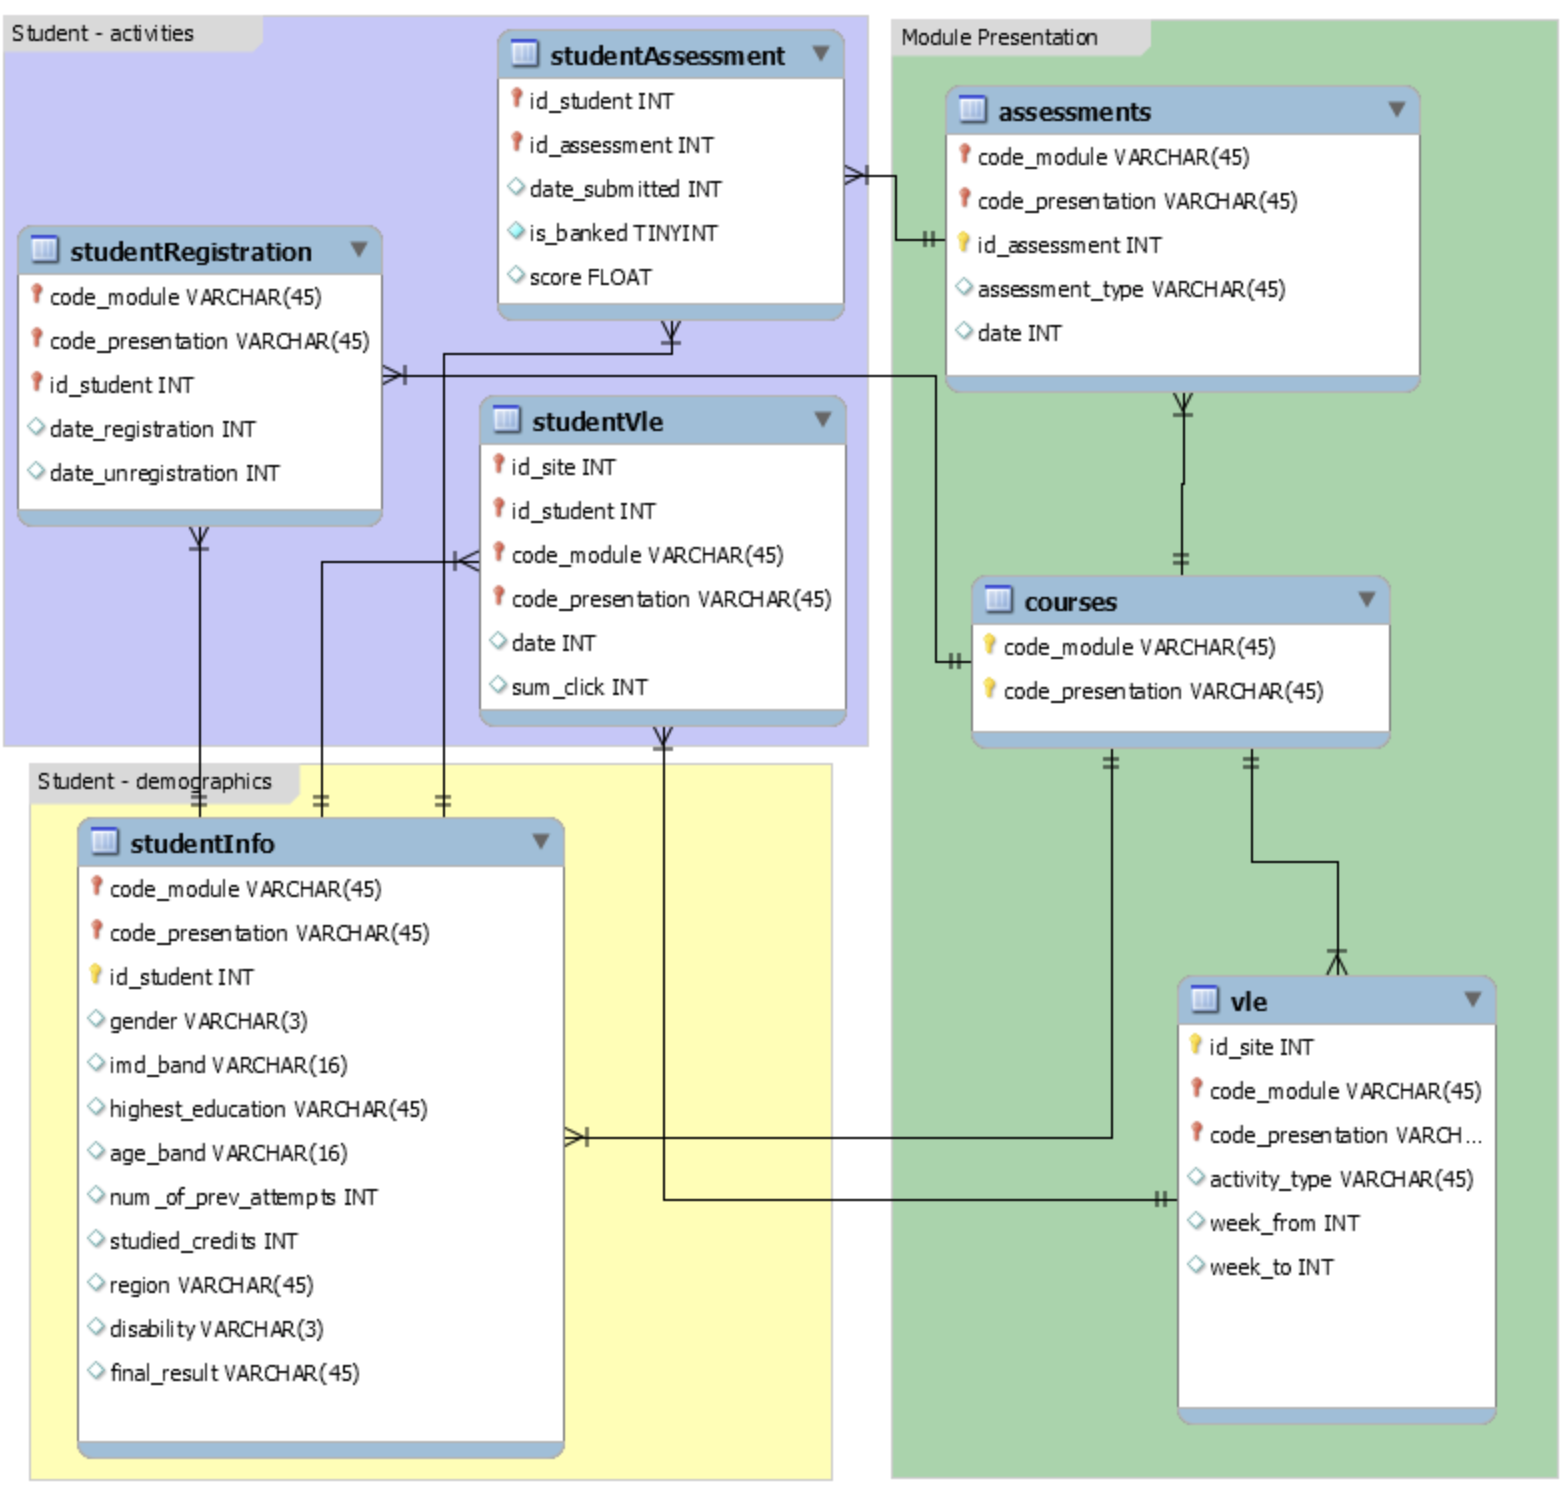
\includegraphics[width=\linewidth]{dataset.png} 
	\caption{Dataset Schema}
	\label{fig:schema}
\end{figure}

Firstly, I noticed a couple of very useful features, such as the score in the studentAssessment table, $\&$ the sum\_click feature in the studentVle table.
Therefore I started by grouping the sum\_click and score attributs, thus finding the total number of times a person clicked within the portal through the year \& their average mark. 
From this, I expected higher scores and click counts to perform higher as it is likely they put more effort in. N.b. This is shown in Table \ref{table:Correlations}.
From these, I plotted the data and noticed that it would be worth using a logistic regression model to test this. However, I noticed a poor performance from this data: 42\% accuracy.
Therefore I went back and added more data to my model, with the intention of using as much data as possible so the model can find patterns easier.

I noticed further useful data, like the date submitted feature; with this I can calculate how many days early a student submitted coursework.
Ideally, one would expect more days before submission would result in a larger coursework mark as the student is more prepared and commited.
In addition, I noticed, the assessments have a weighting, given in the assessments table, so I added data further through scaling the data based on the weight, ie their summative mark,
as well as using their formative mark (where their weight is 0). I noticed this gradually improved the performance of my model, so I continued adding further data.
I eventually included almost all of the data available, so I started to look at the data differently so I included the mean, mean absolute deviation, standard deviation, varience etc for the scores of students' coursework.
This therefore can find patterns from extrapolated data to squeeze more patterns out of the schema. I then outputted the correlation matrix, the descriptions of the data \& the pandas scatter matrix.
These showed notable correlations: 

\begin{table}[H]
	\centering
	\begin{tabular}{|l|l|}
		\hline
		Feature                    & Correlation \\ \hline
		assessment\_var              & -0.208126 \\ \hline
		student\_Std                 & -0.186952 \\ \hline
		assessment\_mad              & -0.185294 \\ \hline
		assessment\_Std              & -0.170608 \\ \hline
		student\_var                 & -0.169245 \\ \hline
		is\_banked                   & -0.163256 \\ \hline
		studied\_credits             & -0.142413 \\ \hline
		num\_of\_prev\_attempts      & -0.095372 \\ \hline
		disability                   & -0.083723 \\ \hline
		assessment\_Meds             & -0.070066 \\ \hline
		student\_mad                 & -0.069468 \\ \hline
		gender                       & -0.028173 \\ \hline
		age\_band                    & 0.060998  \\ \hline
		imd\_band                    & 0.100306  \\ \hline
		highest\_education           & 0.123420  \\ \hline
		assessment\_Mean             & 0.145892  \\ \hline
		formative                    & 0.162990  \\ \hline
		daysEarly                    & 0.176952  \\ \hline
		sum\_click                   & 0.267279  \\ \hline
		summative                    & 0.276203  \\ \hline
		summativeNonScaled           & 0.286314  \\ \hline
		score                        & 0.356086  \\ \hline
		student\_Meds                & 0.359332  \\ \hline
		totalCoursework              & 0.360867  \\ \hline
		\end{tabular}
		\caption{Correlations}
		\label{table:Correlations}
\end{table}

The most surprising of these is the age feature; personally, I would have thought the correlation would have shown a strong negative correlation.
However this may be because the age data values are estimated medians. To improve this correlation, I would need actual data rather than these estimates. 

See the scatter figure in \ref{fig:scatterMatrix}, which plots most data against itself, so people can spot patterns easier. Clearly, features such as score show a positive correlation.
However it is hard to see the correlations against final result as it is a discrete value.

\begin{figure}[]
	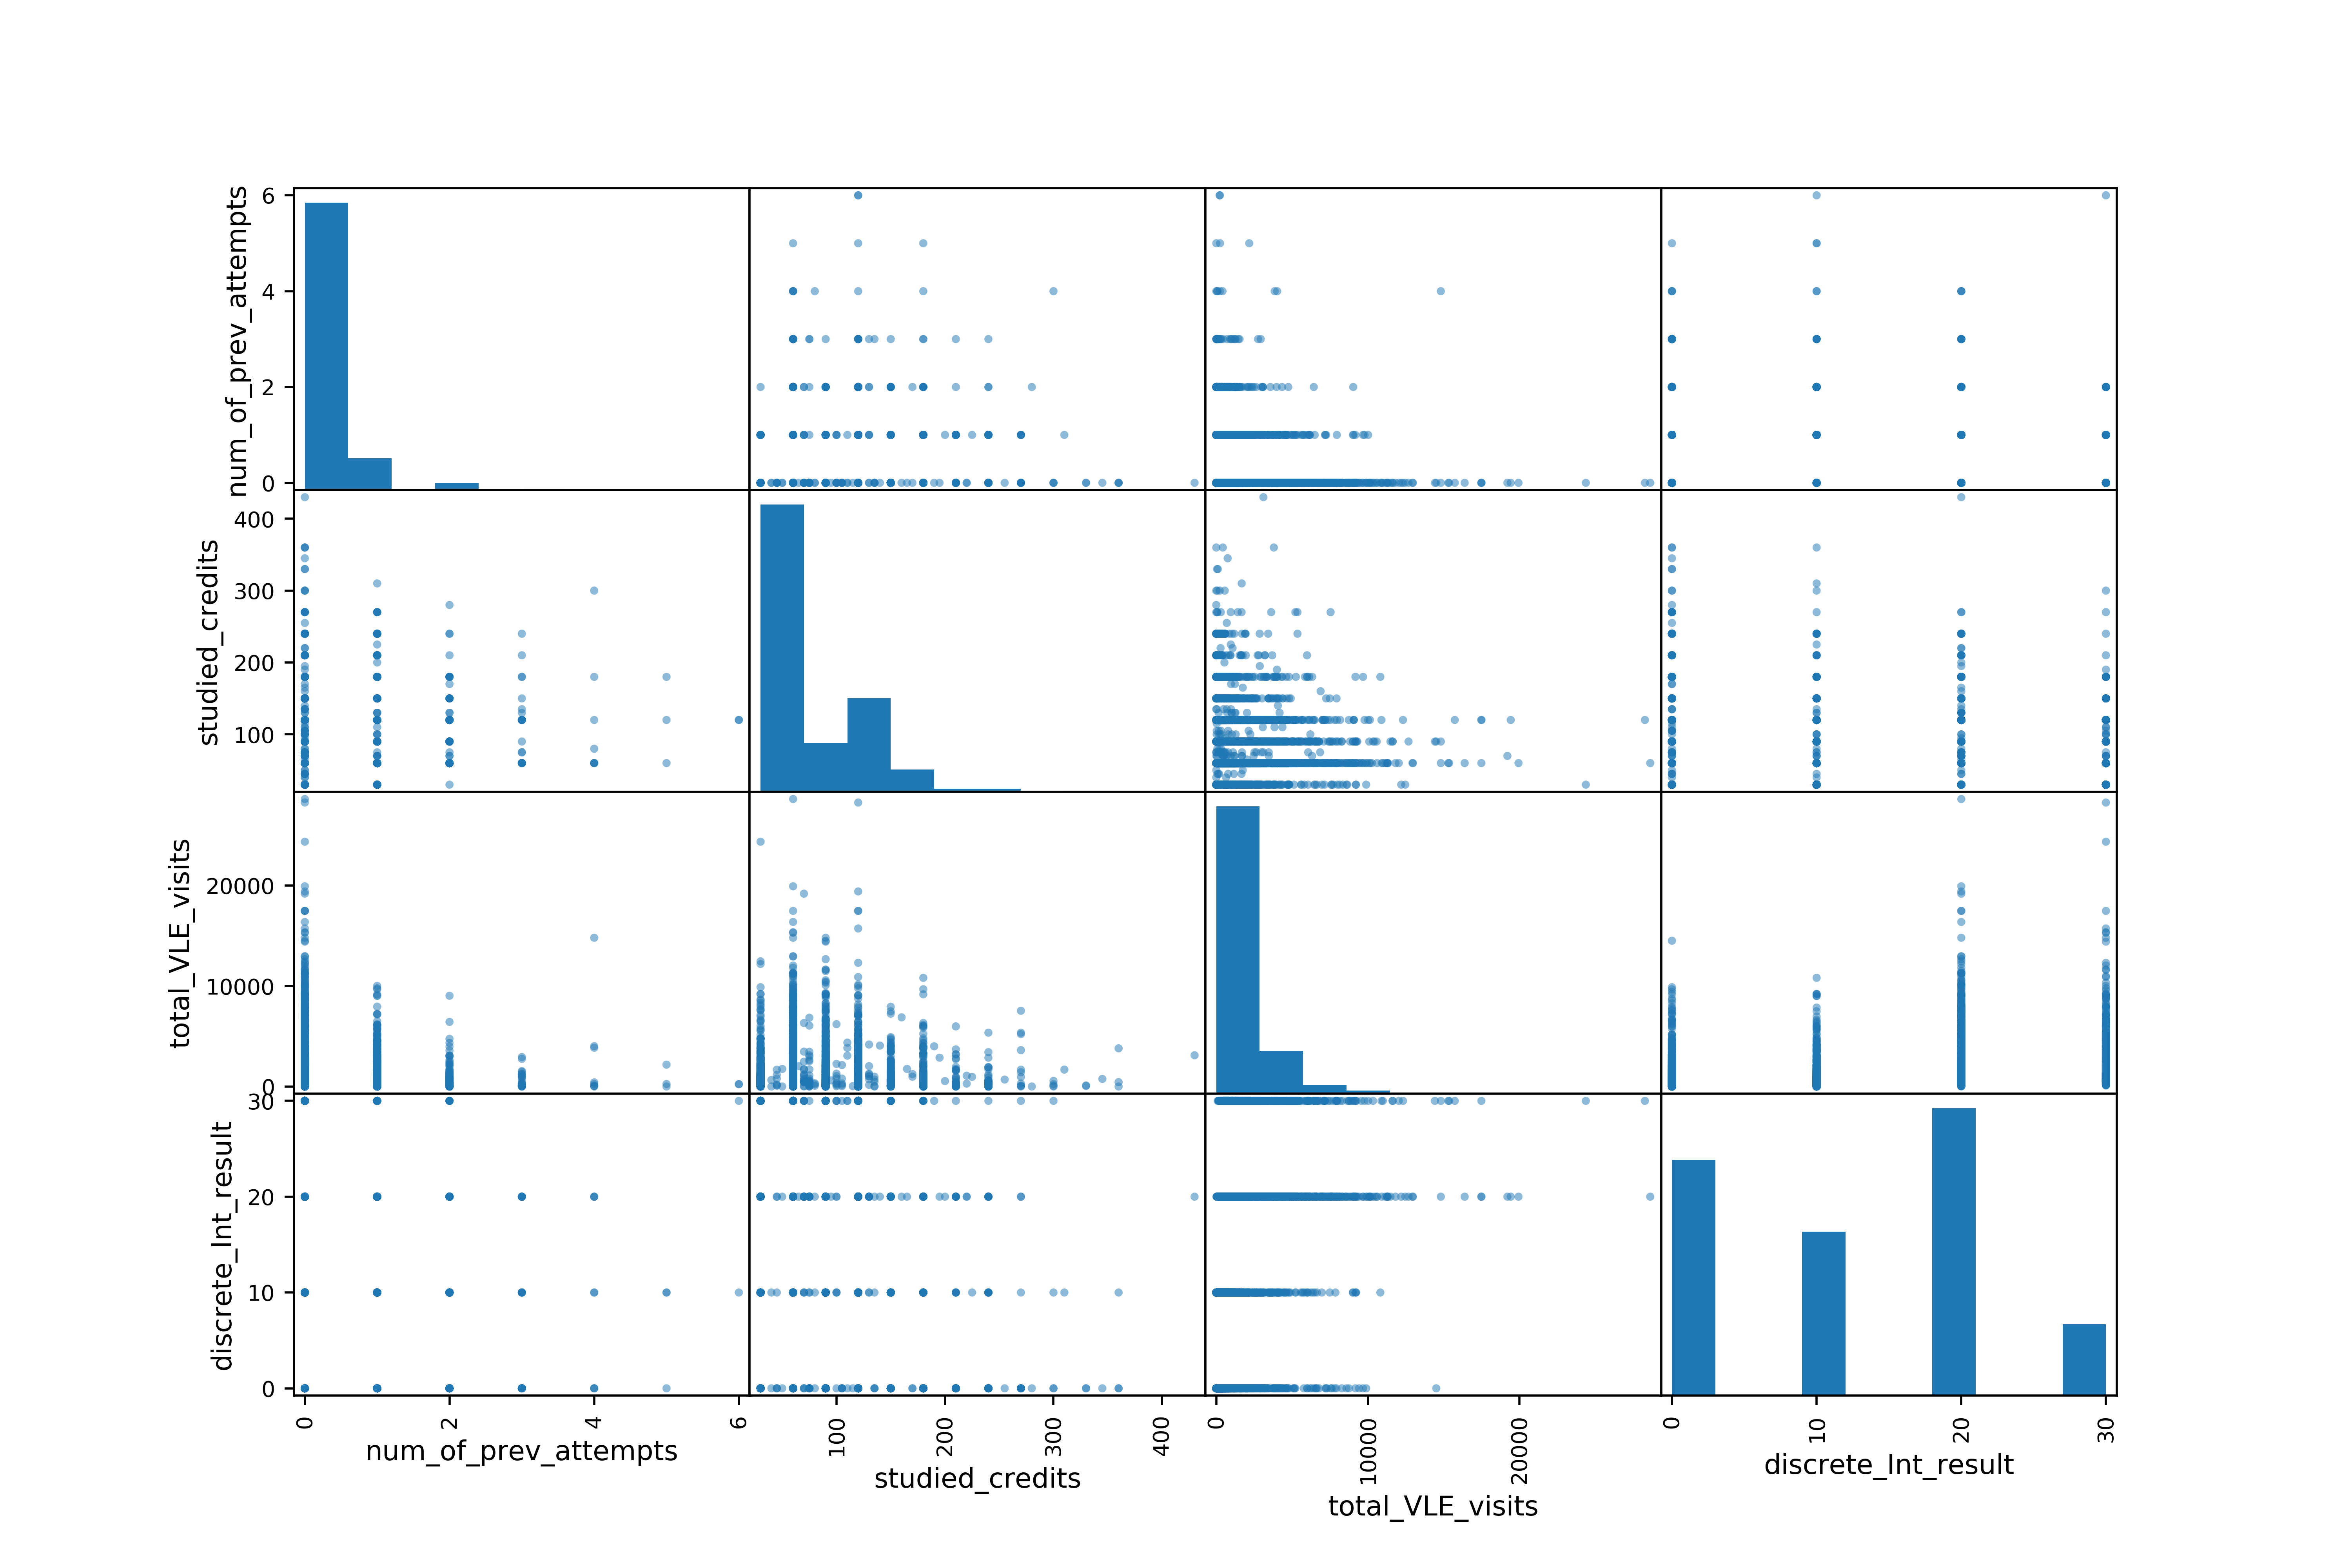
\includegraphics[width=2\linewidth]{Correlation} 
	\caption{Data Scatter Matrix}
	\label{fig:scatterMatrix}
\end{figure}


After data gathering, I looked at preprocessing the data, through using an imputer and normalisation. The imputer changes all NA values to the median of that feature. 
While the normaliser, changes the scale of all features to be within $0-1$, this prevents feature domination with large ranges and makes the features unit dependent
Further, I exchanged certain features to their corresponding categorical codes, so the model can interpret the data.\vfill
\vspace*{13cm} \section{Model Selection}

The following phase was model selection. Here, I first split the data into train and test data this was a 75/25 split; then I tested the Linear, Logistic, SVR (Linear Kernel), SVR (Polynomial Kernel), Decision Tree, \& Random Forrest Regression models, and compared how these performed in cross validation on the training data.

I noticed, the decision tree was the worst performing, with a mean accuracy of 0.15\% between the cross validation folds, this therefore would be a poor model to pick. Next, the linear and SVR (linear kernel) regression models performed at 0.38\% \& 0.35\% respectively. This is expected upon analysing the data, showing little features with a linear correlation.
The SVR (polynomial kernel) performed a little better at 0.45\% accuracy, but instead, I picked the best two performing models: the logistic \& random forrest regression models. These had accuracies of 0.65\% and 0.53\% respectively. 



\section{Model A - Logistic Regression}

After I picked logistic regression, I began my hyperparameter tuning. For this model, I decided to use a grid search to validate the best parameter within the permutations I provided. 
I gave the model, two potential sets of permutations, the first, cycled through the C value, which is the regularisation strength; smaller values show a stronger strength, 
so I started with a strong logarithmic scale to check through, until after enough testing I used the range between 950 and 1125. It also cycled through the tolerance value with small values around the default of 0.0001.
The other set of permutations loop through a similar set of values of C and adjusts the max number of iterations model uses to fit the data and find patterns.

\section{Model B - Random Forest Regressor}

Following my logistic hyperparameter tuning, I tuned my random forrest regressor, using a random search. This randomly picks n permutations to validate the model against based on the given parameters.
I decided to check the number of estimators (trees in forrest), the max depth of each tree in the forrest, the minimum number of samples required at a leaf node, \& the minimum number of samples required to split an internal node.
As the random search prefers ranges, all of these values are provided with the python range type so it can pick any value within the range. This lead to picking 20 out of 244,800 permutations of parameters.

\section{Conclusion}

\begin{table}[H]
	\centering
	\begin{tabular}{l|l|l|}
	\cline{2-3}
												   & Logistic & Random Forrest \\ \hline
	\multicolumn{1}{|l|}{Max Err}                  & 3.000                     & 2.682                           \\ \hline
	\multicolumn{1}{|l|}{Explained Var} 		   & 0.361                     & 0.604                           \\ \hline
	\multicolumn{1}{|l|}{Mean Abs Err}       	   & 0.393                     & 0.405                           \\ \hline
	\multicolumn{1}{|l|}{Mean Square Err}          & 0.513                     & 0.309                           \\ \hline
	\multicolumn{1}{|l|}{RMSE}   				   & 0.716                     & 0.556                           \\ \hline
	\multicolumn{1}{|l|}{Med Abs Err}    		   & 0.000                     & 0.318                           \\ \hline
	\multicolumn{1}{|l|}{r2 Score}                 & 0.343                     & 0.604                           \\ \hline
	\multicolumn{1}{|l|}{Best Score}               & 0.678                     & 0.590                           \\ \hline
	\end{tabular}
	\caption{Metrics of Final Models}
	\label{table:metrics}
\end{table}

In conclusion, the logistic regression model finished with an accuracy of 0.68\%, whereas the Random Forrest Model finished with an accuracy of 0.59\%, therefore making the logistic model initially more desirable.
Upon further inspection and validation on the testing data set, the maxiumum error was 0.3 lower for the random forrest, \& the r2 score was 0.25 higher for random forrest, potentially making random forrest overall a better choice.

\section*{Appendix}
\centering
\begin{figure}[H]
	\includegraphics[width=0.95\linewidth]{age_band_linear_model.png} 
	\caption{Age band against Final Result Linear Regression Model}
	\label{fig:AgeLin}
\end{figure}
\centering
\begin{figure}[H]
	\includegraphics[width=0.95\linewidth]{sum_click_SVR_linear_model.png} 
	\caption{Total VLE clicks against Final Result SVR (Linear Kernel) Regression Model}
	\label{fig:clickSVRLin}
\end{figure}
\centering
\begin{figure}[H]
	\includegraphics[width=0.95\linewidth]{score_linear_model.png} 
	\caption{Score against Final Result Linear Regression Model}
	\label{fig:scoreLinear}
\end{figure}



% \begin{figure}[H]
% 	\includegraphics[width=\linewidth]{score_linear_model.png} 
% 	\caption{Score against Final Result Linear Regression Model}
% 	\label{fig:scoreLinear}
% \end{figure}
	
\end{document}

% assessment_type_mean         -0.248565
% assessment_var               -0.208126
% student_Std                  -0.186952
% assessment_mad               -0.185294
% assessment_Std               -0.170608
% student_var                  -0.169245
% is_banked                    -0.163256
% studied_credits              -0.142413
% num_of_prev_attempts         -0.095372
% disability                   -0.083723
% assessment_Meds              -0.070066
% student_mad                  -0.069468
% gender                       -0.028173
% sum_click_assessment_med     -0.018983
% sum_click_assessment_var     -0.010792
% sum_click_assessment_std     -0.006387
% sum_click_assessment_mad      0.001471
% sum_click_assessment_mean     0.004230
% sum_click_student_var         0.008521
% module_presentation_length    0.032159
% sum_click_student_std         0.055647
% age_band                      0.060998
% imd_band                      0.100306
% highest_education             0.123420
% sum_click_student_mad         0.126426
% sum_click_student_med         0.140700
% assessment_Mean               0.145892
% formative                     0.162990
% daysEarly                     0.176952
% sum_click                     0.267279
% summative                     0.276203
% summativeNonScaled            0.286314
% score                         0.356086
% student_Meds                  0.359332
% totalCoursework               0.360867
% final_result                  1.000000
% Name: final_result, dtype: float64
%             gender  highest_education     imd_band     age_band  \
% count  9524.000000        9524.000000  9524.000000  9524.000000   
% mean      0.545149           1.687211    47.358253    31.350798   
% std       0.497984           0.727579    27.660604     9.413924   
% min       0.000000           0.000000     5.000000    25.000000   
% 25%       0.000000           1.000000    25.000000    25.000000   
% 50%       1.000000           2.000000    45.000000    25.000000   
% 75%       1.000000           2.000000    75.000000    45.000000   
% max       1.000000           4.000000    95.000000    60.000000   

%        num_of_prev_attempts  studied_credits   disability  final_result  \
% count           9524.000000      9524.000000  9524.000000   9524.000000   
% mean               0.140172        74.024570     0.101113      1.685741   
% std                0.440503        39.847497     0.301494      0.870993   
% min                0.000000        30.000000     0.000000      0.000000   
% 25%                0.000000        60.000000     0.000000      1.000000   
% 50%                0.000000        60.000000     0.000000      2.000000   
% 75%                0.000000        90.000000     0.000000      2.000000   
% max                5.000000       430.000000     1.000000      3.000000   

%        sum_click_assessment_var  sum_click_assessment_mean  \
% count               9524.000000                9524.000000   
% mean                  74.516777                   3.955064   
% std                   33.422305                   0.490147   
% min                   32.067263                   2.693114   
% 25%                   38.498765                   3.441819   
% 50%                  102.589812                   4.366362   
% 75%                  102.589812                   4.382149   
% max                  108.934159                   4.382149   

%        sum_click_assessment_mad  sum_click_assessment_med  \
% count               9524.000000               9524.000000   
% mean                   3.671006                  1.984989   
% std                    0.731191                  0.061035   
% min                    2.040295                  1.190639   
% 25%                    2.869737                  2.000000   
% 50%                    4.287328                  2.000000   
% 75%                    4.304819                  2.000000   
% max                    4.304819                  2.000000   

%        sum_click_assessment_std  sum_click_student_var  sum_click_student_std  \
% count               9524.000000            9522.000000            9522.000000   
% mean                   8.282267              84.850854               7.777983   
% std                    2.172846             405.665823               4.935219   
% min                    5.654995               0.000000               0.000000   
% 25%                    5.778362              24.630319               4.962894   
% 50%                   10.115436              53.981253               7.347193   
% 75%                   10.115436              92.102446               9.597002   
% max                   10.419782           29014.287611             170.335808   

%        sum_click_student_mad  sum_click_student_med  \
% count            9524.000000            9524.000000   
% mean                3.715521               1.570349   
% std                 1.464672               0.508601   
% min                 0.000000               1.000000   
% 25%                 2.767893               1.000000   
% 50%                 3.667623               2.000000   
% 75%                 4.508355               2.000000   
% max                30.413223               5.000000   

%        module_presentation_length    is_banked  assessment_Mean  \
% count                 9524.000000  9524.000000      9524.000000   
% mean                   257.927026     0.107938        75.553800   
% std                     12.066254     0.766504         5.533973   
% min                    234.000000     0.000000        58.866817   
% 25%                    241.000000     0.000000        75.662227   
% 50%                    262.000000     0.000000        77.282392   
% 75%                    268.000000     0.000000        78.704859   
% max                    269.000000    12.000000        91.790541   

%        assessment_Meds  assessment_Std  assessment_mad  assessment_var  \
% count      9524.000000     9524.000000     9524.000000     9524.000000   
% mean         80.965034       16.505310       13.609107      347.869158   
% std           4.925141        5.657571        6.004479      349.846195   
% min          68.000000        9.670097        7.657102       93.510774   
% 25%          78.750000       13.786006       10.779208      196.794188   
% 50%          80.333333       14.107937       11.135033      209.484311   
% 75%          82.833333       17.130408       13.516343      305.607739   
% max         100.000000       48.639460       47.835640     2365.797046   

%        assessment_type_mean  totalCoursework  student_Meds  student_Std  \
% count           9524.000000      9524.000000   9520.000000  9145.000000   
% mean               1.097058         9.362033     76.373372    14.235372   
% std                0.494594         4.620329     14.781774     8.177540   
% min                0.000000         1.000000      0.000000     0.000000   
% 25%                0.833333         5.000000     69.000000     8.273268   
% 50%                0.833333         9.000000     79.000000    12.419925   
% 75%                1.333333        12.000000     85.500000    18.006877   
% max                2.000000        28.000000    100.000000    70.003571   

%        student_mad  student_var    daysEarly        score    summative  \
% count  9520.000000  9145.000000  9524.000000  9520.000000  9524.000000   
% mean     10.377955   269.510668   324.758820    75.007182     0.782465   
% std       6.179949   335.464957   314.675464    14.438695     0.818585   
% min       0.000000     0.000000 -1469.000000     0.000000     0.000000   
% 25%       6.000000    68.446970    23.000000    68.333333     0.071875   
% 50%       9.280000   154.254545   279.000000    77.462567     0.697917   
% 75%      13.580270   324.247619   526.000000    84.833333     1.212500   
% max      49.500000  4900.500000  2367.000000   100.000000     9.366333   

%          formative     sum_click  summativeNonScaled  
% count  9518.000000   9524.000000         9524.000000  
% mean     75.243116   2454.264805           57.477716  
% std      24.700125   2468.183061           51.758881  
% min       0.000000      1.000000            0.000000  
% 25%      71.285714    654.000000            6.200000  
% 50%      81.111111   1738.000000           63.500000  
% 75%      89.000000   3519.250000           81.900000  
% max     100.000000  28264.000000          477.190000  
% 75.47956800460815
% Linear: 
% Accuracy:  [0.50474886 0.4843059  0.4794276  0.52886707 0.52424565 0.54550249
%  0.53843081 0.46507239 0.50843098 0.45409406]
% Mean Accuracy Across folds:  0.5033125827504074
% Standard Deviation of the Accuracy Across folds:  0.029915357822658473

% linear regression model against VLE clicks
% Coefficients: 
%  [[2.75398739]]
% Mean squared error: 0.68
% Coefficient of determination: 0.07


% linear regression model against score
% Coefficients: 
%  [[2.14693412]]
% Mean squared error: 0.64
% Coefficient of determination: 0.12


% linear regression model against age band
% Coefficients: 
%  [[0.20092133]]
% Mean squared error: 0.73
% Coefficient of determination: 0.01


% linear regression model against imd band
% Coefficients: 
%  [[0.29918239]]
% Mean squared error: 0.73
% Coefficient of determination: 0.01
% Logistic: 
% Accuracy:  [0.69090909 0.6951049  0.7034965  0.66806723 0.67366947 0.69187675
%  0.67927171 0.67226891 0.67787115 0.67507003]
% Mean Accuracy Across folds:  0.6827605727605729
% Standard Deviation of the Accuracy Across folds:  0.01111622655429652
% SVR - linear kernel: 
% Accuracy:  [0.45282863 0.42123972 0.44179951 0.51572605 0.4590181  0.51082045
%  0.49110263 0.42256805 0.45316717 0.39405953]
% Mean Accuracy Across folds:  0.45623298523534184
% Standard Deviation of the Accuracy Across folds:  0.03767701404860464

% SVR linear regression model against VLE clicks
% Mean squared error: 0.76
% Coefficient of determination: -0.03


% SVR linear regression model against score
% Mean squared error: 0.67
% Coefficient of determination: 0.09


% SVR linear regression model against imd band
% Coefficients: 
%  [[2.55409598e-05]]
% Mean squared error: 0.77
% Coefficient of determination: -0.05
% SVR - polynomial kernel: 
% Accuracy:  [0.53049866 0.50829746 0.49774202 0.56753469 0.49494838 0.57393418
%  0.55132475 0.46299249 0.5246705  0.46188115]
% Mean Accuracy Across folds:  0.517382427344149
% Standard Deviation of the Accuracy Across folds:  0.03755104265435046

% SVR poly regression model against VLE clicks
% Mean squared error: 0.77
% Coefficient of determination: -0.05


% SVR poly regression model against score
% Mean squared error: 0.67
% Coefficient of determination: 0.08


% SVR poly regression model against age band
% Mean squared error: 0.77
% Coefficient of determination: -0.05
% Decision Tree: 
% Accuracy:  [0.61818182 0.60979021 0.64615385 0.64705882 0.64285714 0.60784314
%  0.63445378 0.6232493  0.60784314 0.63865546]
% Mean Accuracy Across folds:  0.6276086658439599
% Standard Deviation of the Accuracy Across folds:  0.015265499869475495
% Random Forrest: 
% Accuracy:  [0.68391608 0.68531469 0.7006993  0.71428571 0.68067227 0.69187675
%  0.68487395 0.68627451 0.68347339 0.69607843]
% Mean Accuracy Across folds:  0.6907465083935673
% Standard Deviation of the Accuracy Across folds:  0.00983815439860965
% 819.8265571594238
% 0.6987236293118646
% {'C': 1100, 'tol': 0.00015}
% 1283.1265239715576
% 0.7121650898121488
% {'n_estimators': 4950, 'min_samples_split': 4, 'min_samples_leaf': 14, 'max_features': None, 'max_depth': 62}
% 10889.761986970901


% Final Logistic Regression Model:
% Max Error: 3.000
% Explained Varience Score: 0.394
% Mean Absolute Error: 0.364
% Mean Square Error: 0.467
% Root Mean Square Error: 0.683
% Median Absolute Error: 0.000
% r2 Score (Accuracy): 0.384
% Best Score: 0.699


% Final Random Forrest Regression Model:
% Max Error: 3.000
% Explained Varience Score: 0.420
% Mean Absolute Error: 0.348
% Mean Square Error: 0.450
% Root Mean Square Error: 0.671
% Median Absolute Error: 0.000
% r2 Score (Accuracy): 0.406
% Best Score: 0.712

% 10891.18006181717